%                                                                 aa.dem
% AA vers. 9.1, LaTeX class for Astronomy & Astrophysics
% demonstration file
%                                                       (c) EDP Sciences
%-----------------------------------------------------------------------
%
%\documentclass[referee]{aa} % for a referee version
%\documentclass[onecolumn]{aa} % for a paper on 1 column  
%\documentclass[longauth]{aa} % for the long lists of affiliations 
%\documentclass[letter]{aa} % for the letters 
%\documentclass[bibyear]{aa} % if the references are not structured 
%                              according to the author-year natbib style

%
\documentclass{aa}  

%
\usepackage{graphicx}
%%%%%%%%%%%%%%%%%%%%%%%%%%%%%%%%%%%%%%%%
\usepackage{txfonts}
%%%%%%%%%%%%%%%%%%%%%%%%%%%%%%%%%%%%%%%%
%\usepackage[options]{hyperref}
% To add links in your PDF file, use the package "hyperref"
% with options according to your LaTeX or PDFLaTeX drivers.
%
\begin{document} 


   \title{The variability  of Betelgeuse explained by surface convection}


    \author{{ Q.~Pilate}\inst{1},{ A.~L{\'o}pez Ariste}\inst{1},{ A.~Lavail}\inst{1},{ Ph. Mathias}\inst{1} }

   \institute{IRAP, Universit\'e de Toulouse, CNRS, CNES, UPS.  14, Av. E. Belin. 31400 Toulouse, France 
             }

   \date{Received ...; accepted ...}

% \abstract{}{}{}{}{} 
% 5 {} token are mandatory
 
  \abstract


   \keywords{
               }

   \maketitle
%
%-------------------------------------------------------------------

\section{Introduction}

Betelgeuse is a prototypical red supergiant (RSG) known to be a semi-regular variable. Several periods can be found in the 
literature usually clustered around the so-called long secondary period (LSP) of 2000 days and other more or less well defined 
periods around 400 and 200 days. Such periods are often linked to radial pulsation modes,   and have been used to model 
the caracteristics of the resonant cavity, hence the size of the star and eventually its evolutionary stage \cite{XXX}.

At the end of 2019, Betelgeuse suffered a sudden and dramatic loss of brightness \cite{}, particularly in the blue colors. 
\cite{Miguel} has demonstrated that such event was due to the emission by the star of a cloud of dust near to the line of sight of 
Earth. In this event it was clear that a change in brightness was not due to any kind of pulsation but to a change on the 
brightness distribution over the stellar disk due to the presence of large quantities of dust. While this may be seen as 
a singular event, it brings up the question whether all changes in brightness cannot be due to similar changes in the brightness 
distribution over the disk. 

Betelgeuse is known to present large convective cells with life times in the order of one to two years and measurable changes 
in the span of one week. Bright convection cells near disk center will increase the integrated brightness of the star when 
compared with other situations where such cells are found near the edges. So even without calling for the formation of 
dust or other changes in opacity, one may argue that the simple convective patterns of the star may create a variability. Such 
variability could be expected to be random, but will present quasi-periodicities related to the typical time scales of the 
convective patterns. 

Since the end of the Great Dimming event, Betelgeuse has continue its random variation of brightness. But the classical periods 
of variation cited above are not visible any more. This may be due to simply the short span of time, that does not afford for 
the peaks to appear prominently in the variability spectra. But it has been sufficient to bring up that other explanation of the variability
in terms  of convective patterns. In order to address this question we seek for the typical periods of 1000, 400 and 200 days in  
observational proxies related to the convective activite but unrelated to pulsations nor directly linked to brightness?

Linear polarization in the atomic lines of the spectra of Betelgeuse, discovered by \cite{auriere_discovery_2016}, has been interpreted as the joint action of 
two mechanisms. First the depolarization of the continuum by atoms which absorb linearly polarized light and re-emit unpolarized light, the 
continuum photons being polarized by Rayleigh scattering. This depolarization produces signals with an azimuth symmetry over the disk that 
would  cancel out the net linear polarization on a homogeneous disk. Thus it must be combined with an inhomogenous disk to produce the net linear polarization 
signal observed. This interpretation suggested the possibility of mapping those brightness inhomogeneities. This has been done by \cite{lopez_ariste_convective_2018} 
even producing 3-dimensional images of the atmosphere of Betelgeuse \citep{lopez_ariste_three-dimensional_2022} when taking advantage of the different height of formation of 
different lines in the spectrum of Betelgeuse. The images produced compare very well with cotemporaneous images made with interferometric 
techniques and show clear convective patterns. Linear polarization in the atomic lines is therefore a proxy of convection, unrelated to radial 
pulsations but linked to the brightness inhomogeneities due to the convective patterns in Betelgeuse. If one can find the aforementioned periods 
in linear polarization, we must conclude that these periods are related to the convective activity which originates those linear polarization 
and unrelated to any radial pulsation phenomena.



\section{Method: Searching for periodicities in the polarization spectra of Betelgeuse}

Betelgeuse has been observed for the last 13 years with Narval and Neo-Narval at the Telescope Bernard Lyot. These instruments measure the polarization 
over the visible spectra of Betelgeuese (390-1000 nm) with high spectral resolution (R=65000) and high polarimetric sensitivity. Despite 
this sensitivity, the signal-to-noise ratios are not sufficient to measure the weak polarization signals in the individual atomic lines of the 
spectrum. These amplitudes are today known to be of the order of $10^{-4}$ times the continuum intensity, and only excepcionnaly do they 
reach amplitudes of $10^{-3}$ the continuum. In these exceptional observations, enough photons can be accumulated per spectral bin to 
see the linear polarization signal above noise \citep{auriere_discovery_2016}. Most commonly, the amplitudes of linear polarization are below noise levels. In those 
occassions we have to add up the signals of thousands of lines to reduce the noise and increase the signal-to-noise ratios. This line addition 
is done through a technique called Least-Squares Deconvolution (LSD) \citep{donati_spectropolarimetric_1997} and assumes that the 
linear polarization signal is similar 
in all spectral lines up to scale factors in the sampling and amplitude. This technique has been successfully used in the past to measure 
magnetic field distributions over stellar surfaces and it is now used to produce images of the brightness distributions in the photosphere 
of Betelgeuse and other red supergiants as cited in the Introduction. 

In this work we shall look into the signals produced through these line-addition techniques, and which produce a pseudo-spectral line in intensity 
and linear polarization which does not belong to any atomic species in particular but to an average of all of them present and emitting in the 
photosphere of Betelgeuse. These signals carry the coherent signals present in the photospheric lines, but the particularities of this or 
that spectral line are erased. All these data has been presented before by \cite{auriere_discovery_2016}, \cite{mathias_evolution_2018} and 
\cite{lopez_ariste_three-dimensional_2022}, which also give details on observing times and conditions as well as more detailed description 
on the data reduction \footnote[1]{Beyond a 2-year proprietary embargo, and up to technical issues, all these data is available through 
PolarBase (http://polarbase.irap.omp.eu/).}



\subsection{Lomb-Scargle periodogram}

Trying to find periods in an astrophysical context can be difficult due to the unevenly spaced observed data. To overcome this issue, 
we used the Lomb-Scargle (hereafter LS) periodogram \citep{lomb_least-squares_1976,scargle_studies_1982}. For a given set of data, it fits sinusoid functions 
using least-squares at each frequency between the first and the last observation. The better the fit, the higher the power attributed to the frequency. 
Since Betelgeuse has been observed by the Télescope Bernard Lyot since 2013, we have ten years of data. Betelgeuse was observed every two or three weeks by 
the spectropolarimeters Narval and Neo-Narval, except during summer. From all these data, we computed the LSD profiles of Stokes I, U and Q. 
The linear polarization present in Betelgeuse is attributed to brightness inhomogeneities, which are due to the convective cells 
present at the surface \citep{lopez_ariste_convective_2018}. Hence, if we are able to find periodicities in the LS periogogram of the LSD profiles of Betelgeuse,
the periodicities would be associated to surface convection. 

To recover variability of Betelgeuse, 
we computed the LS periodogram at each wavelength of the LSD profile, between -25 km/s and 80 km/s. We choose those velocity to span the entire 
signal present in the LSD profile. In the work of \cite{lopez_ariste_convective_2018}, the most blueshifted signal was present at -20 km/s, 
corresponding to the maximal velocity of the rising plasma. The most redshifted signal was 40 km/s. This velocity corresponds 
to the velocity of the star in our reference frame. This last velocity is very important in our study. Signal above 40 km/s is attributed to either huge
convective cells falling back to Betelgeuse, or to rising plumes of plasma located in the hidden face of Betelgeuse,
that rise so high that they appear above the limb.


\subsection{Before and after the dimming}

At the beginning of 2020, Betelgeuse reached a historical minimum in its luminosity, called the great dimming \citep{guinan_fall_2020}. 
From interferometric data, we know that this event was caused by a cloud of gas in front of the line of sight \citep{montarges_dusty_2021}. 
Interferometric images show a huge drop in luminosity in the southern hemisphere of Betelgeuse, leading to this dimming. Interestingly, 
it has been shown by \cite{jadlovsky_analysis_2023} and \cite{dupree_great_2022} that the periodicity of Betelgeuse has changed after the dimming. Using the light curves from AAVSO, 
the authors showed that before the dimming, the dominant period of Betelgeuse was around 400 days. However, after the dimming, this period has changed and 
is now shorter, around 200 days. It means that, after the dimming, there was a change in the behaviour of the atmosphere of Betelgeuse: the period is now
shorter than before the dimming. Our analysis is based on this change of periodicity.

By computing the LS periodogram for each frequency 
in the LSD profile, we expect to find periodicities around the LSP, but also on the 400 days and 200 days period. If the LS periodogram finds a periodicity at a
given wavelength, it would appear as a strong LS power. However, we expect a change in the periodicity after the dimming. 
This would lead to a decrease in the Lomb-Scargle power. By comparing LS periodogram before and after the dimming, we expect to see a change in the LS power,
especially at the 400 days period. 

Figure \ref{LS intensity},\ref{LS Q},\ref{LS U} and \ref{LS linear polarization} show the Lomb-Scargle periodogram of the LSD profile of respectively 
the intensity, stokes Q, stokes U and the linear polarization. The abscissa is the frequency (in $\mathrm{days^{-1}}$), while the ordinate is the heliocentric radial velocity in km/s. 
For each figure, the upper panel is the LS periodogram with data taken before the great dimming of Betelgeuse, that is from 2013 to the beginning of 2019. 
The lower panel is the LS periodogram for the data before and after the dimming: from 2013 to 2023. The white dashed lines represent the different 
periods found in the literature: the LSP at 2000 days, the fundamental pressure mode at 400 days and its first overtone at 200 days. The Lomb-Scargle 
power is normalised. The colorbar indicates the quality of the fit: red areas correspond to good fits from the LS periodogram.

\begin{figure}[!h]
    \centering
    \includegraphics[width=0.5\textwidth]{Lomb-Scargle Intensity.png}
    \caption{Lomb-Scargle periodogram of the LSD profile of intensity. 
    The upper pannel is the LS periodogram for data before the great dimming while the lower panel is the periodogram from the all dataset.
    The ordinate refers to the velocity in the heliocentric radial velocity in km/s. The abscissa is the period in $\mathrm{days^{-1}}$. 
    The three white dashed lines represent respectively (from left to right) the LSP at 2000 days, the 400 days period and its first overtone at 200 days. 
    The Lomb-Scargle power refers to the quality of the fit from the LS periodogram. }
    \label{LS intensity}
\end{figure}

\begin{figure}[!h]
    \centering
    \includegraphics[width=0.5\textwidth]{Lomb-Scargle Stokes Q.png}
    \caption{Same as figure \ref{LS intensity} for stokes Q. }
    \label{LS Q}
\end{figure}

\begin{figure}[!h]
    \centering
    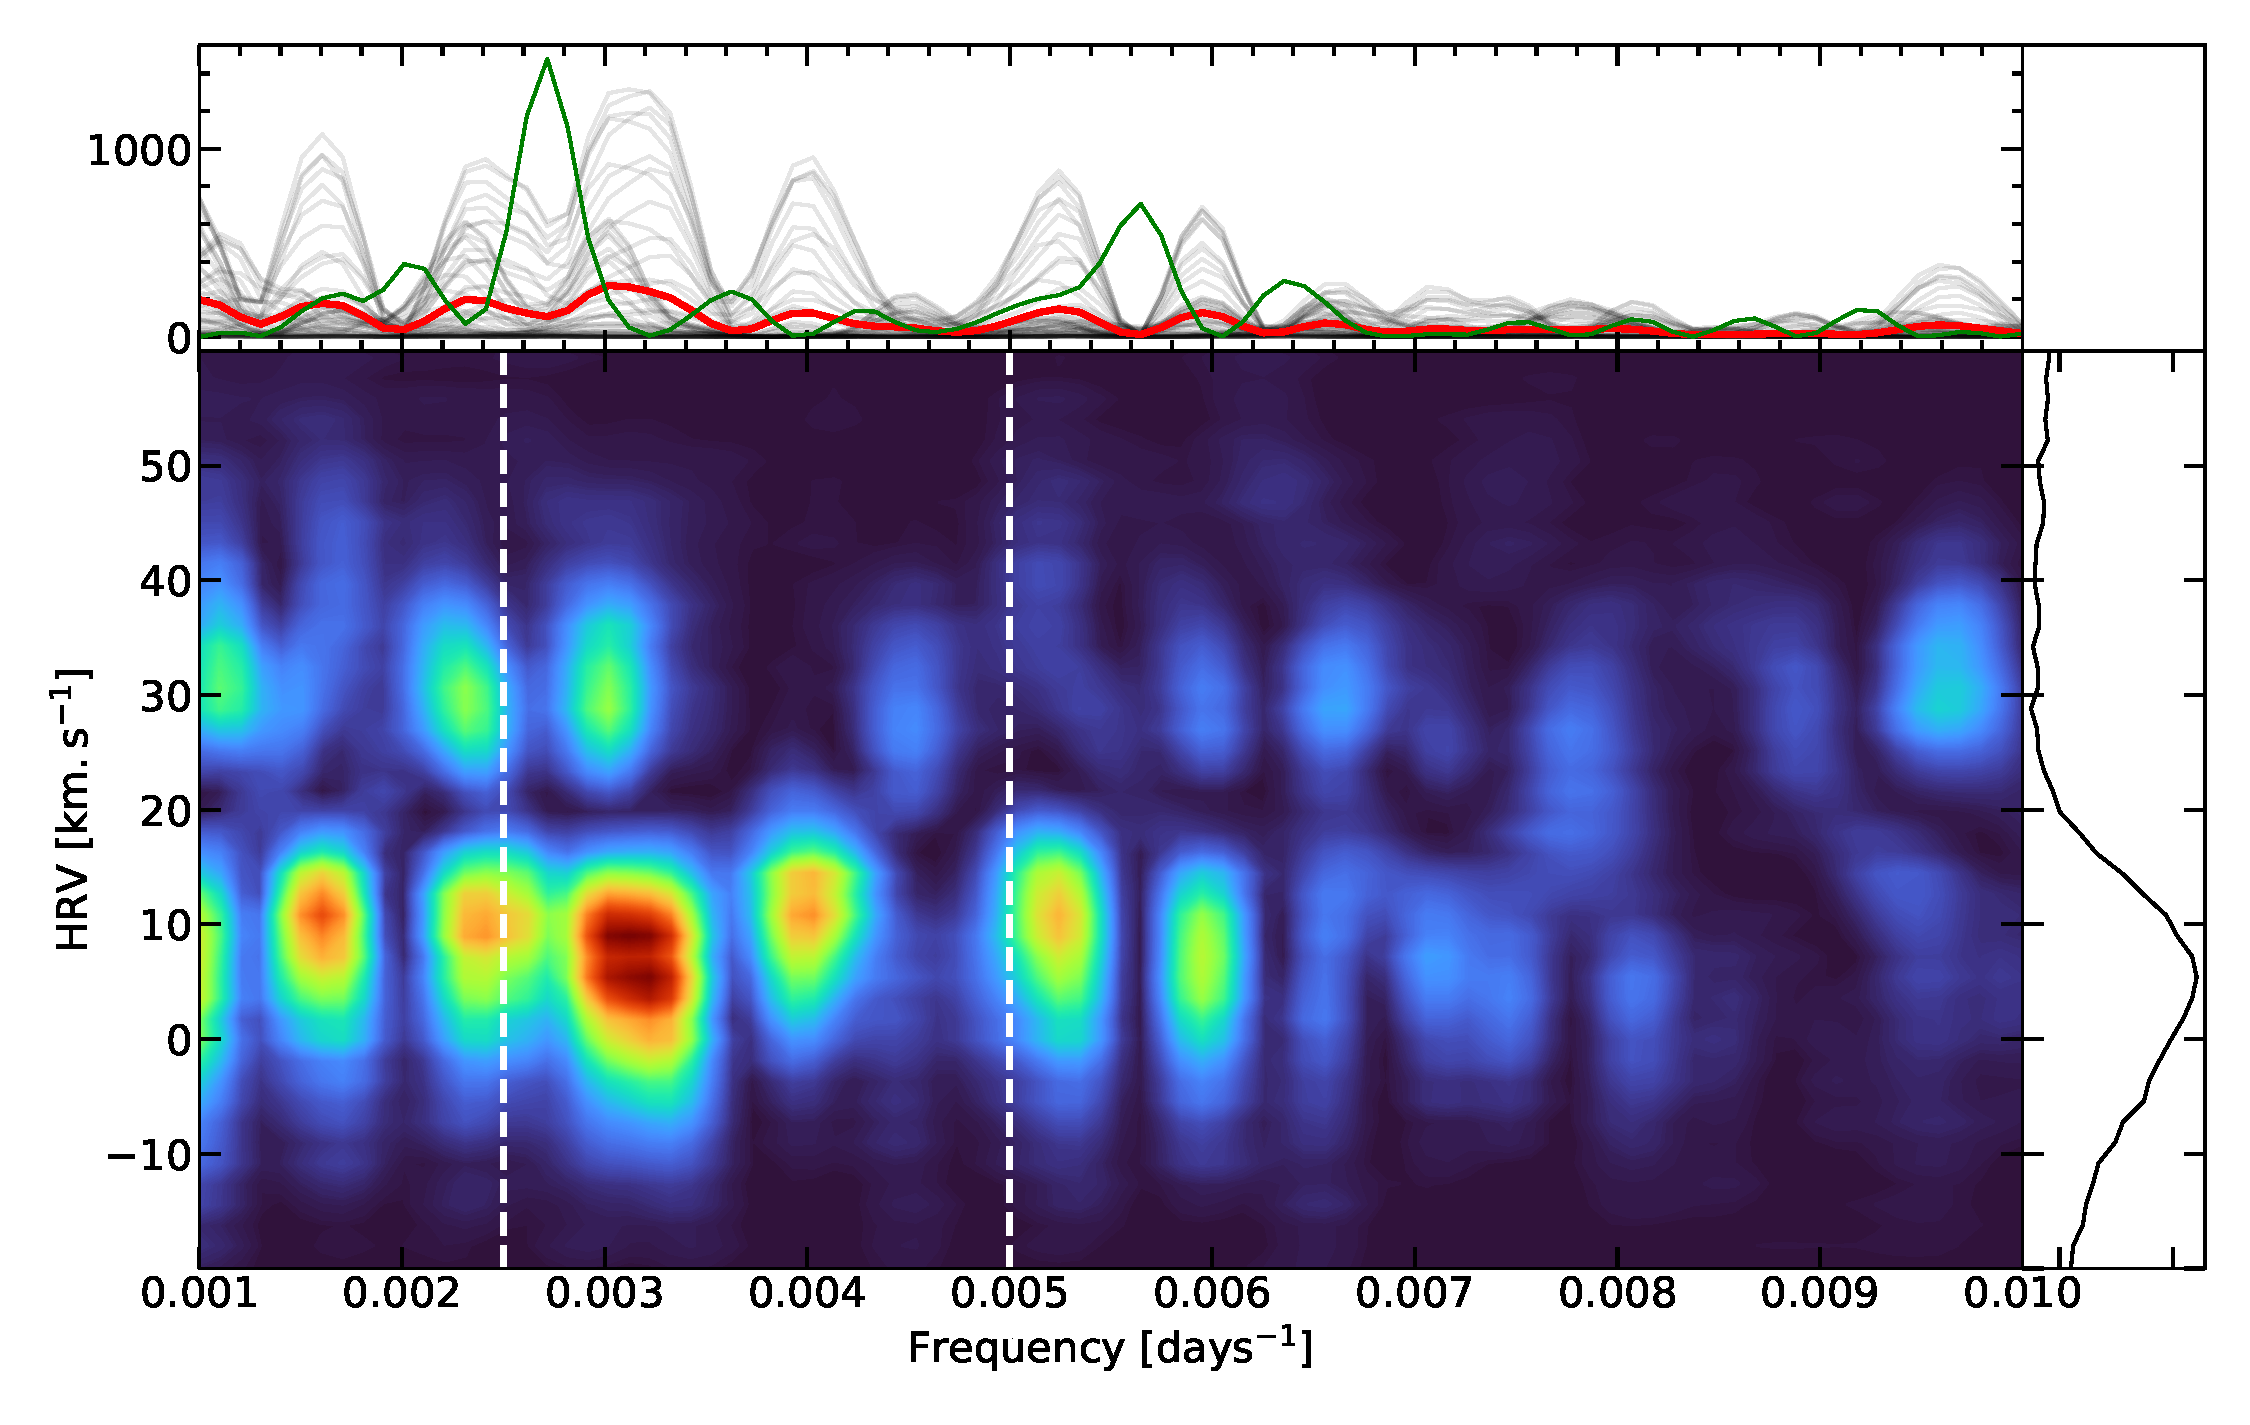
\includegraphics[width=0.5\textwidth]{Lomb-Scargle Stokes U.png}
    \caption{Same as figure \ref{LS intensity} for stokes U.}
    \label{LS U}
\end{figure}


\begin{figure}[!h]
    \centering
    \includegraphics[width=0.5\textwidth]{Lomb-Scargle linear polarization.png}
    \caption{Same as figure \ref{LS intensity} for the linear polarization: $\sqrt{\mathrm{Q^2}+\mathrm{U^2}}$.}
    \label{LS linear polarization}
\end{figure}



\section{Recovering the variability of Betelgeuse in the LSD profile}

\subsection{Intensity}
Figure \ref{LS intensity} shows the LS periodogram of the LSD of the intensity profile. Interestingly, we recover the LSP at 2000 days, 
located at a HRV of $\sim$ 20 km/s. This periodicity seems to change after the dimming, where it is located at a HRV between 0 and 10 km/s. 
There is also a weaker signal at the fundamental mode, around 400 days. This signal completely disappears after the dimming. It is hard to attribute 
this LS power to a periodicity of Betelgeuse, however it might be a hint that this periodicity has changed after the dimming. Furthermore, our results 
in the intensity profile are consistent with the one from \cite{mathias_evolution_2018} who used 2D fourier analysis and found that the dominant period was the LSP. 


\subsection{Stokes Q and U}

Figure \ref{LS Q} and \ref{LS U} show the LS periodogram of both stokes Q and U. It is clear that the LS periodogram is completely different 
from the intensity one. A strong signal is present in fig. \ref{LS Q} around 200 days. Once again, this signal is weaker after the dimming.
Concerning stokes U in fig. \ref{LS U}, it appears that we only recover the LSP, which once again, is weaker after the great dimming. 
Those periodograms rise a lot of questions: why is the 200 days period only present in stokes Q? Why not in stokes U or intensity? 
We will discuss about those questions in the next section. However, it also appears that stokes Q is not sensitive to the LSP, or to be more precise, 
it is much more sensitive to the 200 days period. From this, we can conclude that stokes Q evolves on a time scale much more closer to the first overtone 
mode than the LSP or even the fundamental mode. Because stokes Q is sensitive only to shorter periods, the variation of stokes Q come from another mechanism 
than the one from intensity. Linear polarization in Betelgeuse is due to convective cells, we attribute the signal present in the periodogram 
as the lifetime of convective cells. This is what we observe in the LSD profile of Betelgeuse: from a week to another it does not change that much. 
However, after a few month, the LSD profile of Betelgeuse has completely changed, due to the evolution of convective cells at the surface. 
This would explain the strong signal present at 200 days in stokes Q. 


\subsection{The linear polarization}

Figure \ref{LS linear polarization} shows the LS periodogram of the linear polarization of Betelgeuse: $\sqrt{\mathrm{Q^2+U^2}}$. 
Interestingly, the LS periodogram shows a strong power at 400 days and 2000 days. This signal is much more weaker after the dimming.
While the LSP is already present in the LS of intensity, here we recover the 400 days periodicity, often invoke in the literature. 
Nonetheless, the period is present at a HRV of around 40 km/s. We recall that this velocity is the velocity of the star. 
Every signal above this velocity is either due to the plasma sinking in Betelgeuse, or plumes of plasma rising above the limb of the star, 
as seen in other red supergiant like $\mu$ Cep \citep{lopez_ariste_height_2023}. Up to this point, we want to pinpoint the two elements that are a clue 
to understand the variability of Betelgeuse: the 400 days period is present in the linear polarization signal and also at a HRV above 40 km/s.
In any case, from the linear polarization and the intensity profile, we recover the different periods of Betelgeuse. Since linear polarization is 
associated to convection and because we recover the periods of Betelgeuse, the main mechanism behind the variability of Betelgeuse points toward surface convection.

\subsection{The variability of Betelgeuse inferred from polarimetry imaging}

Using linear polarization, \cite{lopez_ariste_convective_2018} have been able to reconstruct images of Betelgeuse that have been sucessfully compared 
to inteferometric images of \cite{montarges_close_2016}. The images are produced by finding the brightness distribution that better fits the observed linear 
polarization LSD profile using Marquardt-Levemberg minimisation.

Betelgeuse is observed every two weeks by the TBL, hence,
we were able to follow its surface activity through polarimetry imaging. This allowed us to estimate the size and the life time of the convective cells
at the surface. From our images, we computed a quantity called the photo-center, which is sensitive to the size and the number of convective cells. 
An homogeneous star will have a photo-center displacement close to the barycenter of the star, whereas a star with one or two huge convective cells will have a
photo-center displacement more important, up to a few percent of the stellar radius in the case of RSG \citep{chiavassa_probing_2022}. 

Since the photo-center is linked to surface convection, 
we computed the LS periodogram of the displacement of the photo-center. If we recover the different periods from our images, we would
be able to explain them by involving only convection, since our imaging model does not involve pulsations. However, before going further, we have to be carefull with the interpretation of our images. 
Linear polarization suffers from a $180 ^\circ$ degree ambiguity already mentioned in \cite{auriere_discovery_2016}. For that reason, our images can be 
rotated by $180^\circ$ degree, and the brightness distribution will still fit the observed LSD profile. Thus, to obtain a continuity between our images, 
for a given day, we use the brightness distribution of the previous day to start fitting the LSD profile. This is mandatory to obtain a continuity between the images. For the first image, we start with a 
random brightness distribution as the beginning of the fit. Even though we are able to produce images which are consistent with each other, it is important 
to keep in mind that the photo-center displacement will be affected by the choice of the first image. To overcome this issue, we decided to compute
the photo-center displacement from 100 different initial parameters. So that we recover properties that are independent of the choice of the first image. 

\begin{figure}[!h]
    \centering
    \includegraphics[width=0.5\textwidth]{Lomb-Scargle Photo-center.png}
    \caption{Lomb-Scargle periodogram of the 100 photo-center displacement of Betelgeuse. Each blue curve corresponds to a LS periodogram of one photo-center
     displacement. The black line is the average of the 100 LS periodogram. The black dashed lines represent the 2000, 400 and 200 days period respectively 
     (from left to right). The upper panel is the LS from data before the dimming. The lower panel is the LS from the all dataset, 
     including data after the great dimming. }
    \label{LS photocenter}
\end{figure}

Figure \ref{LS photocenter} shows the LS periodogram of each photo-center displacement (blue lines) and the average LS periodogram of the photo-center displacements (black line). 
The upper panel is the LS from the images before the great dimming of Betelgeuse, whereas the lower panel is the LS for the whole set of data, 
including after the dimming. The black dashed lines are the 2000, 400 and 200 days period respectively. First, we find the the LS power is high around the LSP.
We also notice a decrease in the Lomb-Scargle power before and after the dimming. It appears that there are two smalls bumps around the 400 days period. 
Those bumps almost disappear after the dimming. Even though it is hard to attribute the 400 days variability to those bumps, from polarimetry imaging,
we still find that there is a difference before and after the dimming. However, in our case, our images only involve surface convection.
The LS of the photo-center displacement point toward a variability explained by convection only. The photo-center only is not enough to attribute the variability
of Betelgeuse to surface convection, but what we found from polarimetry imaging is consistent with what we obtained from linear polarization.
Both the photo-center displacement and the LS of the linear polarization point toward a variability explained by surface convection.  




\section{Surface convection to explain variability}

\subsection{The 400 days period explained by rising plumes of plasma}

In the previous section, we have seen that we recover the different period of Betelgeuse from the intensity and linear polarization signal. 
While the nature of the LSP is still in debate, the nature of the lower periods is attributed to pulsations of the pressure modes 
(e.g \cite{kiss_variability_2006}). The mechanism behind the pulsation of Betelgeuse is attributed to the $\kappa$-mechanism. In this section, we attempt to 
find an explanation to the 400 days periodicity of Betelgeuse. As mentioned before, the LS periodogram of linear polarization shows a periodicity 
around 400 days. Furthermore, the region where the LS power is high is around 40km/s. This wavelength corresponds to most redshifted signal present in Betelgeuse.


The polarization signal is supposed to remain between -20 and 40km/s. Signal above 40km/s is associated to plasma rising behind the limb of Betelgeuse. 
This scenario has been observed in the RSG $\mu$ Cep and was introduced by \cite{lopez_ariste_height_2023} to explain the excess of linear polarization beyond 
the velocity of the star. In $\mu$ Cep, the linear polarization signal is very strong and often present, whereas in Betelgeuse, the signal above the 
velocity of the star is less strong. However, because it is present from time to time, the LS periodogram finds this signal above the limb and interprets it as a
periodic signal at this wavelength of 40 km/s. Hence, the strong power associated to this wavelength might be due to those convective plumes that are 
rising above the limb from time to time. From this scenario, we can explained the 400 days period in the light curve. From time to time,
Betelgeuse is ejecting plasma in the interstellar medium due to winds. The plasma can be ejected from the hidden face of Betelgeuse. 
It rises so high that we see the rising plume from the Earth, because the plume rises above the limb of the star, contributing to the linear polarization signal. Hence, from Earth, 
the signal associated to this plume appears redshifted compared to the velocity of the star. This plume increases the number of photons that we receive,
leading to an increase of the brightness. After a few weeks or months, the plume falls back to Betelgeuse, disappearing from our point of view, 
leading to a decrease of the brightness.
This is exactly what we see in the LSD profile of the linear polarization of Betelgeuse: 
from time to time, there is a net signal above 40km/s, which is present for a few weeks, and then disappears. Since this signal is not always present, 
it is found by the LS periodogram as a periodic event. However, it is not periodic at all: because the plumes rise at random moments, sometimes they 
appear every years, sometime they do not. This would explain why we only see it before the dimming. After the dimming, this kind of event never happened 
for the moment. Thus, the LS periodogram, at that precise frequency, finds that there is a periodic signal before the dimming, but not after, leading to
a lower LS power at this frequency.

Concerning the 200 days period, it is caused by the timescale on which the stokes parameters evolve. For instance, the 
LSD profile of stokes Q or U will slightly change if we observe Betelgeuse every two weeks. However, on a longer timescale, for example a few month, 
the LSD profile of stokes Q and U will change a lot. They are directly linked to the dynamics of the surface, hence,  their variation scale the lifetime 
of convective cells. Some convective cells can live up to a few month, leading to this peak in the LS periodogram of stokes Q. As showed by
\cite{lopez_ariste_convective_2018}, some convective cells can live up to years, explaining also the LSP. One can notice that the peak is not present in stokes U, which might be due to stochastic event. 
However, if we try to explain the periodicity of Betelgeuse using pulsations, we would see this signal in either stokes U and the linear polarization. 


To summarise what we have done so far: we were able to explain the variability of Betelgeuse using surface convection only. The convective cells play 
the most important role in the variability of Betelgeuse. Our work does not need pulsation to explain its variability. This does not mean that there are 
no pulsation in Betelgeuse. What we claim is that the most important factor in the variability of Betelgeuse is the timescale on which the convective 
cells evolve. Pulsation could exist on Betelgeuse, but they are not the main contributor to the variability. 

\subsection{The variability of the light curve of Betelgeuse}

In the literature, it is reported that before the great dimming, the main period of Betelgeuse was 400 days \citep{kiss_variability_2006}. 
This pulsation is associated to the fundamental model of pressure modes. After the dimming, this period is shorter and is now around 200 days, 
associated to the first overtone of the fundamental mode. However, there are no explanations concerning this change of variability due to the dimming.


Using the data from AAVSO, we studied the light curve of Betelgeuse. Figure \ref{light curve Betelgeuse} shows the light curve of Betelgeuse in the visible, 
from 2014 up to now. Before the great dimming, the magnitude of Betelgeuse evolves on a timescale of a year, whereas after the dimming, the variability of Betelgeuse has changed. It is clear from fig. \ref{light curve Betelgeuse} that the 
variability of Betelgeuse is evolving on a timescale shorter than one year. However, from middle 2023 up to now, the magnitude of Betelgeuse remains almost 
constant, which is not consistent with a pulsating scenario. The constant magnitude of Betelgeuse points toward another scenario than pulsation. Using surface 
convection, we can fully explain the variability of Betelgeuse. The oscillations in the light curve are due to two mechanisms: surface convection and rising 
plumes of plasma beyond the limb of the star. This last mechanism being random, it happens from time to time. The timescale on which convective cells evolve
is between one and two years, which is also consistent with the 400 days period found in the literature.  After the dimming, the change of periodicity in the
light curve is explained by surface convection, the random variation of brightness distribution could lead to the 200 days periodicity found in the literature. 
The constant brightness of Betelgeuse for the last 6 months is explainable by the same random brightness distribution: the surface of Betelgeuse is calm, 
leading to this constant brightness. In the future, we expect to see the light curve of Betelgeuse to change, maybe with another main period, but which 
is in fact caused by surface convection. Thus, the main mechanism in the variability of Betelgeuse is surface convection, which is sufficient to explain the 
variation in the magnitude of Betelgeuse.  


\begin{figure}[!h]
    \centering
    \includegraphics[width=0.5\textwidth]{Light_curve_Betelgeuse.png}
    \caption{Light curve of Betelgeuse from AAVSO in the V-band.}
    \label{light curve Betelgeuse}
\end{figure}


\section{Conclusion}

\begin{acknowledgements}
    This work was supported by the "Programme National de Physique Stellaire" (PNPS) of CNRS/INSU co-funded by CEA and CNES.
    We acknowledge support from the French National Research Agency (ANR)
    funded project PEPPER (ANR-20-CE31-0002)
    \end{acknowledgements}
    
    \bibliographystyle{aa}
    %\bibliographystyle{aa}
    
    \bibliography{art75}
\end{document}